\section{Problem Setup}
\subsection{Motivating Example}
To motivate our solution, we present a running example scenario inspired by
one of our experimental datasets.
In this problem, an analyst is training a classifier to predict the occurrence 
of seizures based on Electroencephalogram (EEG) and patient data.
\begin{example}
An analyst is given a 15-dimensional feature vector $x \in \mathbb{R}^{15}$ of electrical signals and three binary features indicating risk factors including family history, age, and gender.
The observation is a label $y\in \{0,1\}$ of whether the patient is having a seizure.
The analyst trains an L1-Loss SVM on this data.

Medical records are often dirty due various problems in digitization and data integration \cite{fortunearticle}.
After model training, the analyst is informed of inconsistencies in the three binary features representing patient data.
However, the procedure to determine which patients' data are corrupted requires querying source medical records.
\end{example}
With existing tools, the analyst has a few options: (1) she can ignore the errors and assume that the inconsistencies do not affect the results, (2) she can discard the data and assume that the errors are not correlated with the other covariates, or (3) she can clean the entire dataset and retrain her model.
These solutions pose a dichotomy where either the analyst has to face expensive data cleaning, complete retraining, or cope with the unreliable analysis.
In \sys, we present the analyst with a middle ground where she can initialize the framework with her existing model and iteratively converge towards the clean model.
To optimize the convergence rate, we feed information of each successive model iteration back to prioritize which data to sample.

\subsection{Machine Learning and Loss Minimization}
The SVM model in our example is an instance of parametric Machine Learning.
In parametric Machine Learning, the goal is to learn a set of model \emph{parameters} $\theta$ from training examples.
A common theoretical framework in Machine Learning is empirical risk minimization with linear predictors.
We start with a set of training examples $\{(x_{i},y_{i})\}_{i=1}^{N}$
on which we minimize an loss function $\phi$ at each point parametrized that is parametrized by $\theta$.
\[
 \theta^{*}=\arg\min_{\theta}\sum_{i=1}^{N}\phi(x_{i}^T\theta,y_{i})
\]
For example, in a linear regression $\phi$ is:
\[
\phi(x_{i}^T\theta,y_{i}) = \|\theta^Tx_{i} - y_i \|_2^2
\]
$\phi$ is often designed to be \emph{convex}, essential meaning bowl-shaped, to make the training this model 
tractable.
This class of problems includes all generalized linear models and support vector machines.

Typically, a \emph{regularization} term $r(\theta)$ is added to this problem.
The regularization term $r(\theta)$ is traditionally what is used to increase the robustness of the model.
$r(\theta)$ penalizes high or low values of feature weights in $\theta$ to avoid overfitting to noise in the
training examples.
\[
 \theta^{*}=\arg\min_{\theta}\sum_{i=1}^{N}\phi(x_{i}^T\theta,y_{i}) + r(\theta)
\]
For example, a popular variant of linear regression is called LASSO which is:
\[
 \theta^{*}=\arg\min_{\theta}\sum_{i=1}^{N}\|\theta^Tx_{i} - y_i \|_2^2 + \lambda \cdot \|\theta\|_1
\]
By applying the L1 regularization term, if one of the features is particularly noisy, and does not add predictive value, it will get excluded.

\subsection{Systematic Biases}
As in our example, we consider the case when data is systematically biased.
If we train a model with respect to the incorrect data, while we might have achieve a good out-of-sample accuracy on the incorrect data, the classifications are incorrect in a semantic sense.
Data cleaning gives us information about the ``true" data distribution, which is highly beneficial when errors have systematic biases.
Without cleaning, certain subpopulations of data might be frequently mispredicted. 
The problem that we are interested in is when models are being trained on dirty data but are deployed or tested on clean data (or predicting ``real world" trends).
Two characterize this problem there are two metrics that we look at:

\vspace{0.5em}

\noindent\textbf{Model Error. } Let $\theta$ be the model trained on the dirty data, and let $\theta^*$ be the model trained on the same data if it was cleaned. Then the model error is defined as $\|\theta - \theta^*\|$.

\vspace{0.5em}

\noindent\textbf{Testing Error. } Let $\theta$ be the model trained on the dirty data, and let $\theta^*$ be the model trained on the same data if it was cleaned. Let $T(\theta)$ be the out-of-sample testing error when the dirty model is applied to the clean data, and $T(\theta^*)$ be the test error when the clean model is applied to the clean data. The testing error is defined as $T(\theta^*) - T(\theta)$

\subsection{Data Cleaning on a Budget}

\begin{figure}[t]
\centering
 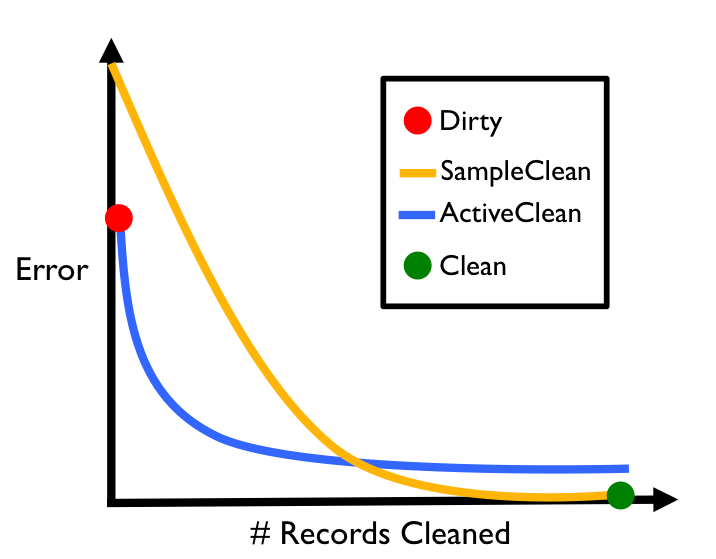
\includegraphics[width=0.6\columnwidth]{figs/arch2.png}
 \caption{\sysfull starts with a dirty model and tries to iterative correct the error in batches. In many datasets, this leads to an improved convergence rate over naive uniform sampling. \label{sys-arch2}}
\end{figure}

Suppose, we have a budget of cleaning $k \ll N$ records of data.
The naive solution is to take a uniform random sample of $k$ records, and apply data cleaning.
This approach was proposed in SampleClean \cite{wang1999sample} for aggregate query processing.
This has a two limitations: (1) most of the sampled data is probably clean so a lot of ``cleaning" effort is wasted and (2) training an accurate model from only $k$ records may be infeasible.
In Figure \ref{sys-arch2}, we illustrate the tradeoff space of sampling and data cleaning.
At two extremes we have no cleaning (just using the dirty data) and full cleaning.
We argue that the naive approach of uniform sampling is not suited for Machine Learning (SampleClean) because it struggles at small sample sizes.
We design \sys to make greater progress at these small sample sizes using the dirty model as an initialization.
\sys potentially sacrifices asymptotic performance if the dirty model is not a good initialization, we may have to take a full cleaning pass through the data to train an accurate model.
We evaluate these tradeoffs extensively in our experiments.

\begin{problem}[ActiveClean Problem]\label{activeclean}\sloppy
Let $R$ be a dirty relation and each row $r \in R$ is 
turned into a feature vector and label tuple $F(r) \mapsto (x,y)$.
We are given a convex regularized loss model parametrized
by $\theta$ trained on the set of features and labels $\{(x,y)\}$.
The user specifies two data cleaning components: (1) error detection
which selects a set of candidate dirty data $R_{dirty}$, and (2) error 
repair which cleans a record $C(r) \mapsto r_{clean}$.
With a budget of applying cleaning i.e., $C(\cdot)$, only k times, we return an estimate $\hat{\theta}$ of the optimal clean model.
\end{problem}

\subsection{Two perspectives on error}
When faced with such errors there are two contrasting perspectives from the Machine Learning and the Database communities.

\vspace{0.5em}

\noindent\textbf{Existing Database Literature. } 
Traditionally, cleaning is agnostic to the queries and analysis that happens downstream. 
This perspective breaks down when cleaning is so expensive that we can only clean a small number of records.
Ideally, we should clean the records that are most valuable to the downstream analysis.

\vspace{0.5em}

\noindent\textbf{Existing  Machine Learning Literature. } The Machine Learning community has focused on
designing models that are robust to outliers (i.e., values far away from the typical value)
For example, in the case of linear regression, we can change the $L_2$ norm to an $L_1$ norm to mitigate the effect of outliers:
\[
\phi(x_{i}^T\theta,y_{i}) = \|\theta^Tx_{i} - y_i \|_1
\]
The quadratic L2 loss implies that examples that deviate far from the typical example are quadratically penalized as opposed to linearly penalized with the L1 loss.
There is a natural tradeoff between robustness and efficiency.
The more robust a technique is, the less efficient it will be (i.e., estimate variance for a fixed number of training examples).
Robust techniques are best suited for random errors that look significantly different the rest of the examples.
When errors are systematic, the Machine Learning answer has been to design features in such a way that they are robust to some systematic bias.
For example, in image processing, scale-invariant feature transforms (SIFT) are widely applied that allow for image models invariant to pose or scaling issues.

\vspace{0.5em}

\noindent\textbf{The \sys Contribution. } We try to bring two perspectives together in this work to address the problem of expensive to clean systematic errors, namely the Database idea of data cleaning and the Machine Learning formalization of empirical risk minimization.
Some errors require expensive cleaning procedures, increasingly using the crowd, and we joint have a time budget on cleaning and analysis.
\sys prioritizes cleaning with respect to an estimated impact on the clean model.


\iffalse

\subsection{SampleClean Project}

Traditionally, data cleaning has explored expensive, up-front cleaning of entire datasets for increased query accuracy.
We proposed the SampleClean problem, in which an analyst cleans a small sample of data, and then estimates the result to an aggregate query e.g., \sumfunc, \countfunc, or \avgfunc.
The main insight from the SampleClean project is that highly accurate answers for aggregate queries does not require cleaning the full dataset.
Generalizing this insight, there is a deep relationship between the application (i.e., the query) and how an analyst should budget their effort in data cleaning.
In fact, \avgfunc and \sumfunc queries are a special case of the convex loss minimization discussed in the previous section:
\[
\phi = (x_{i} - \theta)^2
\]

We then extended the SampleClean work to study cleaning Materialized Views \cite{technicalReport}.
Suppose base data is updated with insertions, deletions, or updates, we explored how we could efficiently propagate
changes to a sample of the view instead of the full view.
Subsequent queries on the view could be answered approximate.

The SampleClean problem inspired an eponymous system that implements sampling, data cleaning, and approximate query processing on the Apache Spark stack \cite{sampleclean}.
Also included in the Apache Spark stack are Machine Learning libraries including MLlib \cite{mllib} and GraphX \cite{graphx}.
The in-memory architecture of the Apache Spark stack allows for increasingly interactive analysis \cite{AgarwalMPMMS13, armbrust2015spark}.
Analysts can prototype data processing workflows on samples to evaluate performance before running expensive batch processing jobs on entire datasets.
With data cleaning and machine learning libraries in the same software ecosystem, we see a new opportunity for joint optimization for interactive model building.



\subsection{Stochastic Gradient Descent}
Sampling is a natural part of any Machine Learning workflow, as stochastic optimization is widely used to fit model parameters.
The problems described in the previous subsections are often trained using a technique called Stochastic Gradient Descent (SGD) or one of its variants.
The basic idea of SGD is to draw a data point at random, calculate the gradient at that point, and then update a current best estimate with that gradient.
\[
\theta^{(t+1)}\leftarrow\theta^{(t)}-\gamma\nabla\phi(x_{i}^T\theta,y_{i})
\]
 SGD can also be applied in a ``mini-batch" mode, where we draw a subset of data $S^{(t)}$ at random and update with the average gradient.
 \[
 \theta^{(t+1)}\leftarrow\theta^{(t)}-\frac{\gamma}{\|S^{(t)}\|}\sum_{i\in S^{(t)}}\nabla\phi(x_{i}^T\theta,y_{i})
 \]

We can use this workflow for designing an anytime data cleaning methodology.
As data is sampled, we can clean the samples.
The analyst then can stop at anytime and use the best model at that instant.
SGD and its variants are well-studied and there are lower-bounds on the convergence rates using these techniques. 
Recently, a number of works have explored non-uniform sampling distributions for stochastic optimization \cite{zhao2014stochastic, qu2014randomized}.
The main insight is that non-uniform distributions may on average estimate the gradient accurately.
In this work, we explore how to design such a non-uniform distribution for iterative data cleaning.

\fi


 